\section{Litterature comparaison}
% Delete the text and write your Discussion here:
%------------------------------------

In order to estimate the veracity of the combined model presented, we propose to compare where possible to published evolution grids from the literature. The Sonora grid published in 2021\parencite{marley_sonora_2021} uses a cloudless atmosphere in chemical equilibrium with an interior model. It covers a compatible domain of planetary masses. The Sonora grid does not consider irradiation and gives radii as a function of effective temperature. As such to compare as accurately as possible, we propose to use the minimal irradiation temperature available (100K) and vary uniquely internal temperature and mass.\par

\begin{figure}
    \centering
    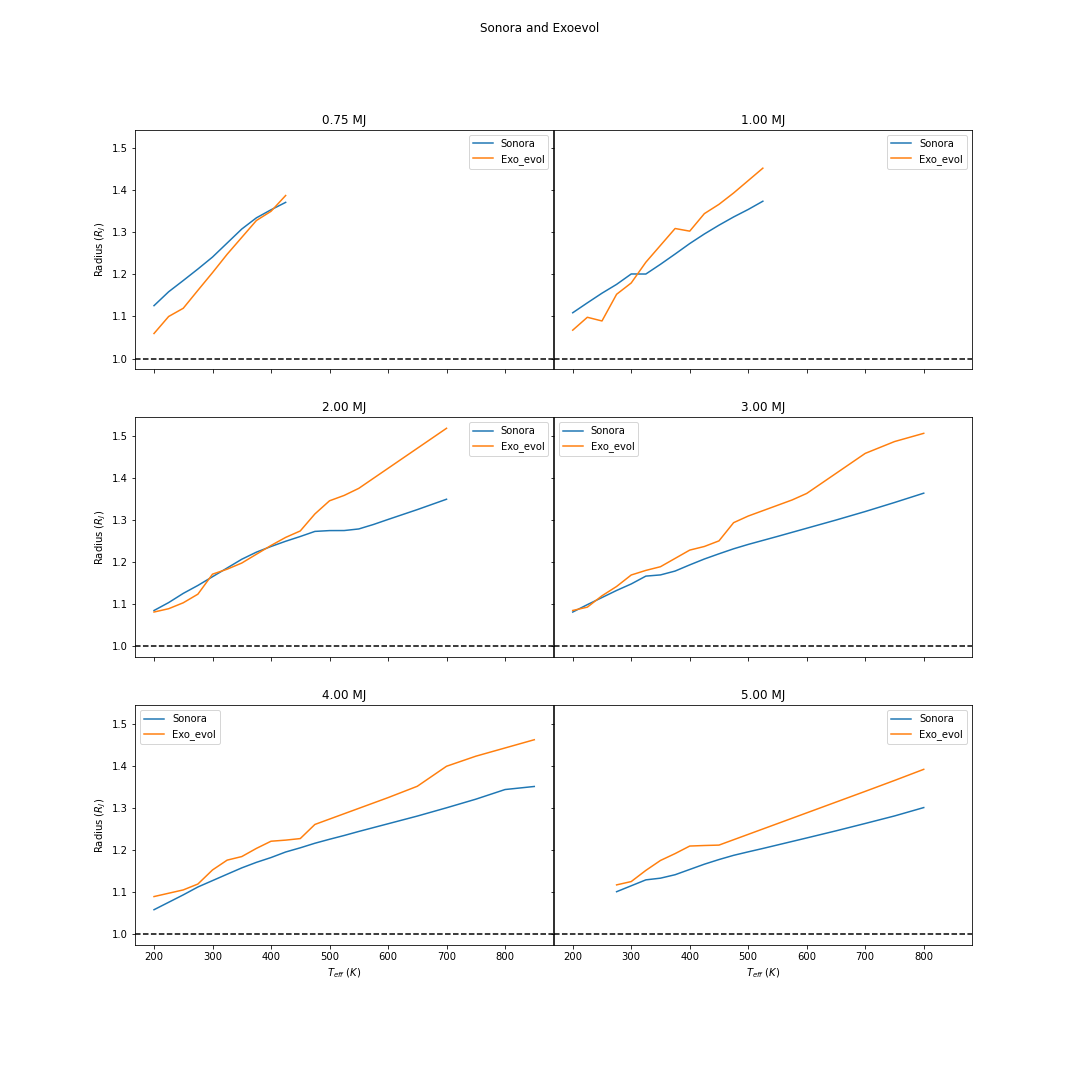
\includegraphics[width=0.48\textwidth]{Images/comp_sonora.png}
    \caption{Sonora and exoevol (exorem+exoris) interpolated to same mass values}
    \label{fig:Son+Exo}
\end{figure}


\begin{figure}
    \centering
    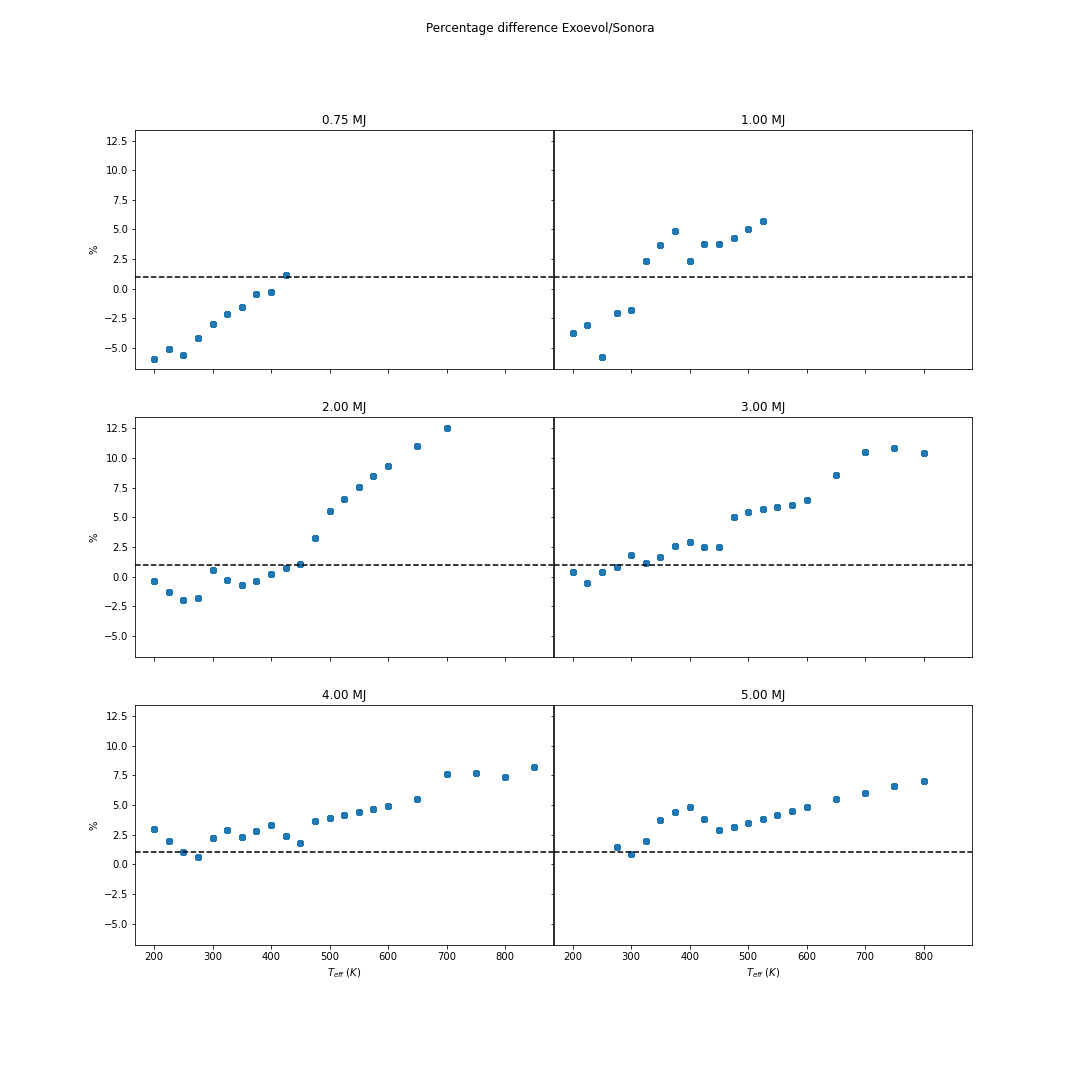
\includegraphics[width=0.48\textwidth]{Images/perc_diff_sonora.png}
    \caption{Percentage difference between Sonora and exoevol (exorem+exoris) at same mass values}
    \label{fig:Son+Exo_perc}
\end{figure}

With \cref{fig:Son+Exo} and \cref{fig:Son+Exo_perc} we see that the difference between the two models remains below around 10\% for the mass and effective temperature range considered. The difference between both models increases with the effective temperature. The differences remain however satisfactory taking into account the at the atmosphere model we use (Exorem) has out of equilibrium chemistry and for the interior model we take into account a core size (10 Earth masses). \par

The Philips et al. model \parencite{phillips_new_2020}  published using the atmo atmosphere model is a useful comparaison as atmo uses an out of equilibrium chemsitry model. Again as irradiation temperature and internal temperatures are not given, we take the non irradiated case (100K irradiation temperature)

\begin{figure}
    \centering
    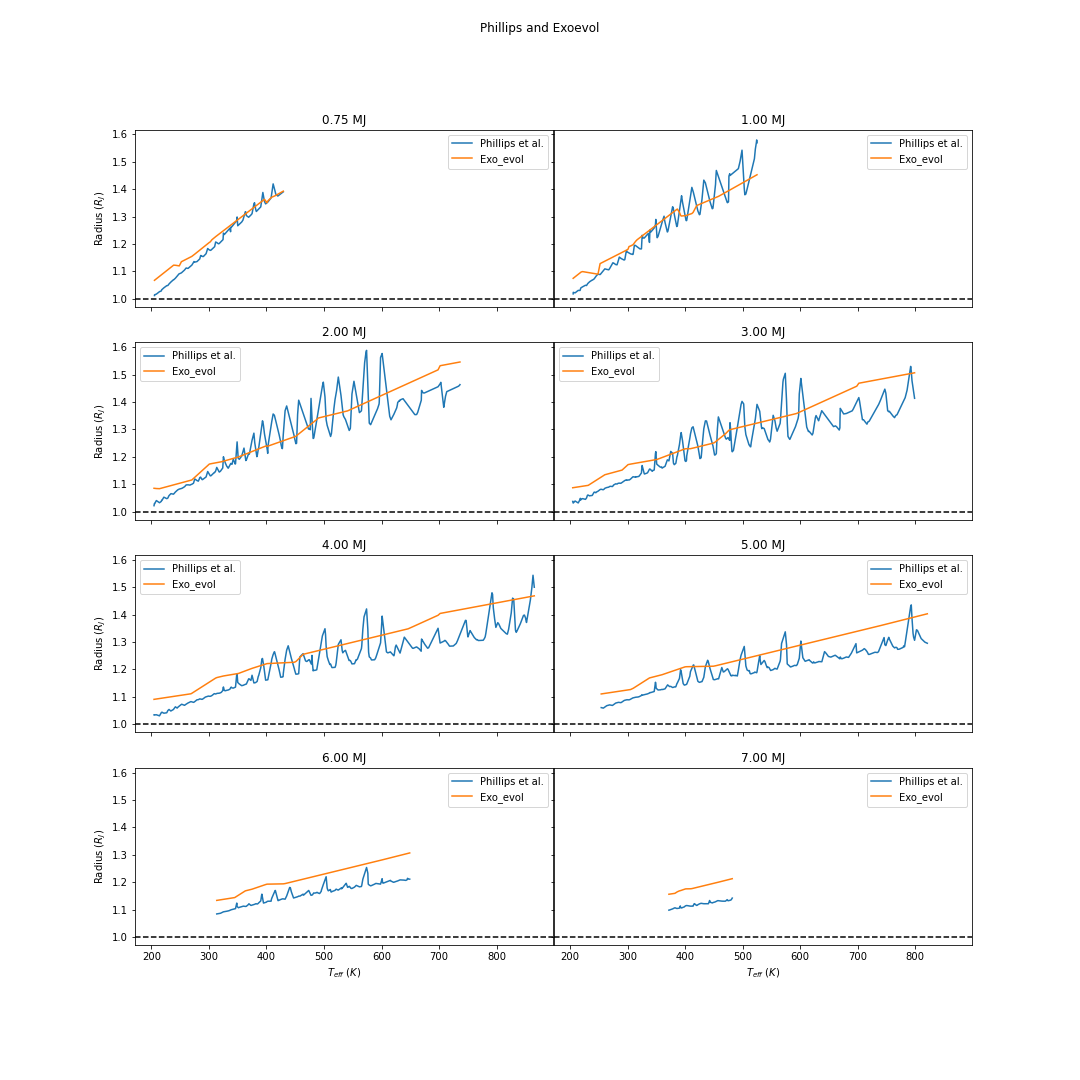
\includegraphics[width=0.48\textwidth]{Images/comp_phillips.png}
    \caption{Phillips et al. and exoevol (exorem+exoris) interpolated to same mass values}
    \label{fig:Phil+Exo}
\end{figure}


\begin{figure}
    \centering
    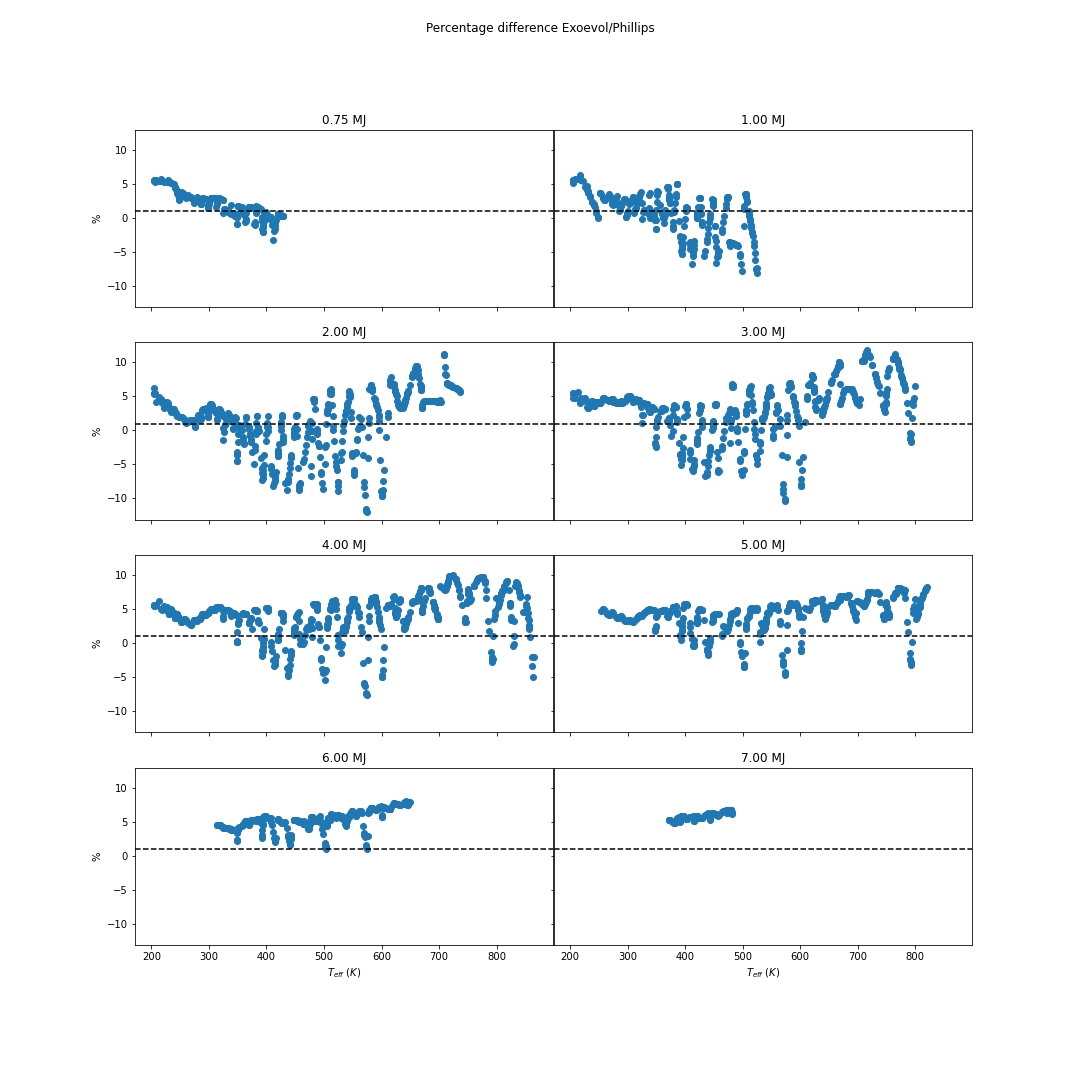
\includegraphics[width=0.48\textwidth]{Images/perc_diff_phillips.png}
    \caption{Percentage difference between Phillips et al. and exoevol (exorem+exoris) at same mass values}
    \label{fig:Phil+Exo_perc}
\end{figure}

(Note oscillations in Phillips et al. data is due to interpolation and requires correcting)

With \cref{fig:Phil+Exo} and \cref{fig:Phil+Exo_perc} we see again that the difference between the two models remains below around 10\% for the mass and effective temperature range considered. The difference between both models is more constant across effective temperature values considered. The choice of the core mass fraction could explain some of the observed differences. A higher core mass than the one considered would lower Exoevol radius closer to that of Philips et al. \par

A comparison transmission spectroscopy is required here.


